% !TeX root = ../main.tex

% REVIEW
\section{Introduzione}
Nei precedenti capitoli sono stati introdotti i concetti alla base della cultura DevOps, del ciclo di vita del processo di sviluppo di applicazioni mobile e delle applicazioni multipiattaforma, arrivando a definire un caso di studio industriale. In questo capitolo viene descritto come è stato effettivamente realizzato il sistema per l'automazione del processo di sviluppo nel rispetto dei requisiti e delle specifiche indicate nel capitolo precedente.

In questa fase di realizzazione del sistema di automazione e di implementazione della pipeline viene considerato il progetto base\footnote{\href{https://github.com/paganellif/DevOps-per-applicazioni-mobile-un-caso-di-studio-industriale/tree/3-applicazioni-multipiattaforma/kmm-example}{https://github.com/paganellif/DevOps-per-applicazioni-mobile-un-caso-di-studio-industriale/tree/3-applicazioni-multipiattaforma/kmm-example}} fornito dal plugin KMM\footnote{\href{https://plugins.jetbrains.com/plugin/14936-kotlin-multiplatform-mobile}{https://plugins.jetbrains.com/plugin/14936-kotlin-multiplatform-mobile}} per Android Studio al fine di mantenere il focus sul processo in modo più agnostico possibile rispetto ad una specifica applicazione utilizzatrice come può essere MaggioliEbook, argomento trattato nel capitolo successivo.

\section{Self-Hosted MacOS GitLab Runner}
Come anticipato nel capitolo \ref{ch:app-multiplatform} tutta la toolchain per lo sviluppo iOS è disponibile solamente per il sistema operativo macOS, il che implica la necessità di un ambiente macOS anche per l'esecuzione della pipeline, almeno per tutti i task riguardanti l'applicazione iOS. Esistono diversi modi per realizzare un sistema di automazione compatibile con i vincoli imposti da Apple e possono essere suddivisi nelle seguenti categorie:

\begin{itemize}
    \item \textbf{Soluzione completa as-a-Service} - Il grande interesse per l'automazione e lo sviluppo di applicazioni iOS da parte delle aziende ha portato alla nascita di servizi cloud dedicati a questo scopo come ad esempio \textit{Bitrise}\footnote{\href{https://www.bitrise.io/home}{https://www.bitrise.io/home}} e \textit{XCode Cloud}\footnote{\href{https://developer.apple.com/xcode-cloud/}{https://developer.apple.com/xcode-cloud/}}.
    \item \textbf{Runner macOS managed} - Un runner, ovvero il componente che esegue effettivamente i task della pipeline, può essere \textit{managed} o \textit{self-hosted}, come descritto nel capitolo \ref{ch:devops}. Nel caso di un runner managed con sistema operativo macOS si evita lo sforzo di configurare e mantenere un componente importante del sistema di automazione ma si hanno costi elevati: solitamente al consumo di risorse di questa tipologia di runner è applicato un fattore moltiplicativo poco sostenibile in termini di costi. Alcuni esempi di piattaforme con questo modello di business per i runner managed sono GitHub Action\footnote{\href{https://docs.github.com/en/billing/managing-billing-for-github-actions/about-billing-for-github-actions\#minute-multipliers}{https://docs.github.com/en/billing/managing-billing-for-github-actions/about-billing-for-github-actions\#minute-multipliers}} e GitLab CI\footnote{\href{https://docs.gitlab.com/ee/ci/pipelines/cicd\_minutes.html\#additional-costs-on-gitlab-saas}{https://docs.gitlab.com/ee/ci/pipelines/cicd\_minutes.html\#additional-costs-on-gitlab-saas}}.
    \item \textbf{Runner macOS self-hosted} - L'altra tipologia di runner consiste nella installazione del componente su una macchina con sistema operativo macOS che deve essere configurata e mantenuta dall'utilizzatore. In questo caso è possibile utilizzare macchine virtuali as-a-Service, come quelle fornite da AWS\footnote{\href{https://aws.amazon.com/ec2/instance-types/mac/}{https://aws.amazon.com/ec2/instance-types/mac/}} (Amazon Web Services), oppure hardware fisico Apple per installare ed eseguire il runner.
\end{itemize}

Data la disponibilità di tutta la toolchain Android per il sistema operativo macOS e il costo nullo in caso di runner self-hosted, è stata scelta quest'ultima tipologia per l'esecuzione dell'intera pipeline. L'installazione e la configurazione di un runner di questa tipologia può essere più o meno complicata in base alle funzionalità necessarie per il sistema di automazione ed è una procedura chiamata registrazione. Nel caso specifico del caso di studio di questo progetto, i principali parametri per la registrazione del runner sono: (\textit{i}) shell executor, (\textit{ii}) token di registrazione al Server CI, (\textit{iii}) cache condivisa e (\textit{iv}) livello di concorrenza.

Definire un executor di tipo \textit{shell} per il runner permette di aprire una nuova shell sulla macchina host per l'esecuzione di ogni job della pipeline e quindi di utilizzare tutti gli strumenti installati sulla stessa macchina. La cache condivisa e il livello di concorrenza permettono invece di ottimizzare il processo parallelizzando l'esecuzione dei task. Il seguente comando bash\footnote{\href{https://github.com/paganellif/DevOps-per-applicazioni-mobile-un-caso-di-studio-industriale/blob/5-automazione-del-processo-di-sviluppo/setup-gitlab-macos-runner.sh}{https://github.com/paganellif/DevOps-per-applicazioni-mobile-un-caso-di-studio-industriale/blob/5-automazione-del-processo-di-sviluppo/setup-gitlab-macos-runner.sh}} mostra i parametri utilizzati per l'installazione e la configurazione del runner GitLab macOS self-hosted su una macchina fisica Apple:

\begin{listing}[H]
    \inputminted{bash}{code/macos-runner-setup.sh}
    \caption{Comando bash per l'installazione e la configurazione del runner macOS self-hosted}
\end{listing}

Il seguente codice\footnote{\href{https://github.com/paganellif/DevOps-per-applicazioni-mobile-un-caso-di-studio-industriale/blob/5-automazione-del-processo-di-sviluppo/config.toml}{https://github.com/paganellif/DevOps-per-applicazioni-mobile-un-caso-di-studio-industriale/blob/5-automazione-del-processo-di-sviluppo/config.toml}} mostra invece il contenuto del file di configurazione del runner, generato in seguito all'esecuzione del comando sopra indicato:

\begin{listing}[H]
    \inputminted{toml}{code/macos-runner-config.toml}
    \caption{File di configurazione (\textit{config.toml}) generato al momento della installazione del runner}
\end{listing}

\section{Modello di branching}
L’utilizzo di un adeguato flusso di lavoro è fondamentale per definire una efficiente automazione CI/CD. Con \textit{branching} si intende l’utilizzo di uno o più flussi principali di lavoro dai quali divergono altri flussi per svolgere determinati lavori per poi convergere al loro termine: in base alle modalità di apertura e chiusura di questi flussi si definiscono diversi modelli di branching.

Il modello che si intende utilizzare (fig. \ref{branching}) è basato sul modello di branching GitFlow\footnote{\href{https://www.atlassian.com/it/git/tutorials/comparing-workflows/gitflow-workflow}{https://www.atlassian.com/it/git/tutorials/comparing-workflows/gitflow-workflow}} e prevede tre branch principali:

\begin{itemize}
    \item \textbf{dev} - Flusso principale di sviluppo. Ogni modifica apportata a questo branch corrisponde al rilascio di una nuova versione \textit{alpha} per la validazione interna. E' da questo branch che vengono aperti e chiusi nuovi branch, sia per lo sviluppo di nuove funzionalità (\textit{feature}) che per la risoluzione di bug/patch (\textit{bugfix}).
    \item \textbf{test} - Branch modificato solamente tramite merge di modifiche provenienti dal branch \textit{dev} con lo scopo di rilasciare una nuova versione \textit{beta} per la validazione esterna.
    \item \textbf{main} - Branch modificato solamente tramite merge di modifiche provenienti dal branch \textit{test} con lo scopo di rilasciare una nuova versione in produzione (\textit{prod}).
\end{itemize}

\begin{figure}[H]
    \centering
    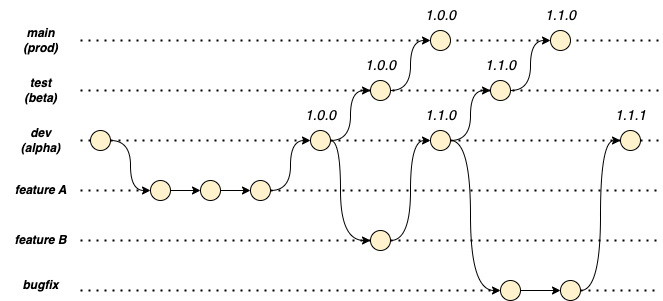
\includegraphics[width=0.9\textwidth]{img/branching-model.png}
    \caption{Esempio di flusso di sviluppo adottando il modello di branching indicato}
    \label{branching}
\end{figure}

Grazie ai meccanismi di automazione a supporto della CI/CD fornite dal CI Server si definiscono specifiche regole di attivazione, chiamate \textit{trigger rules}, che permettono di indicare quando uno specifico job deve essere eseguito. Queste regole si basano su eventi che si verificano sul sistema di versionamento come ad esempio commit, tag e merge request. Tramite questa funzionalità è possibile dunque discriminare quali file sono stati modificati e su quale branch per eseguire le operazioni associate come descritto sopra.

\begin{figure}[H]
    \centering
    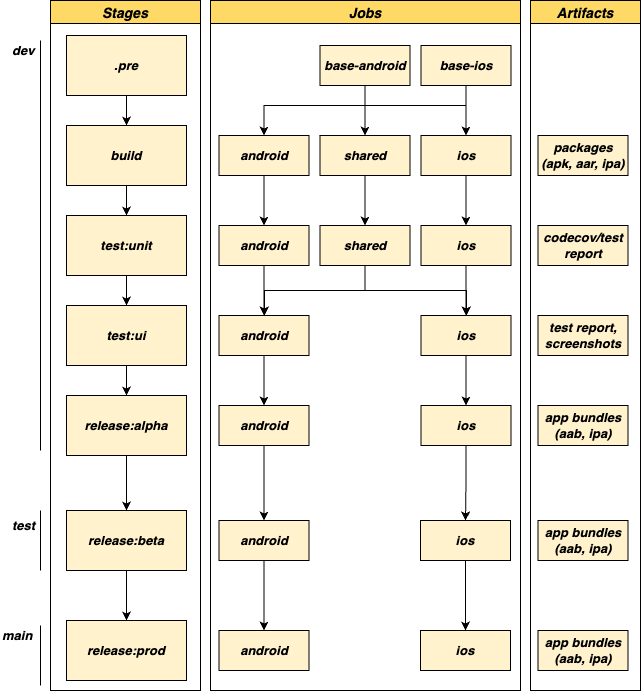
\includegraphics[width=1\textwidth]{img/cicd-branch-jobs.png}
    \caption{Stage, job e artefatti associati agli eventi sui branch che compongono l'intera pipeline}
    \label{pipeline-branches}
\end{figure}

\section{Templating}
Uno dei principali vantaggi del meccanismo Pipeline as Code, anticipato nel capitolo \ref{ch:devops}, è la possibilità di utilizzare metodologie simili a quelle utilizzate nella programmazione per la definizione delle pipeline. Tramite i seguenti costrutti forniti dalla piattaforma GitLab è possibile utilizzare tecniche come ereditarietà e incapsulamento per definire pipeline riutilizzabili, il quale è un importante requisito del processo, definito nel capitolo precedente:

\begin{itemize}
    \item \textbf{Template} - I file YAML che definiscono una pipeline o sottoparte di essa, possono risiedere in un repository diverso da quello in cui si trova il progetto che la utilizza. In questo modo si definisce una sola volta il flusso base per poterlo successivamente includere e/o estendere negli specifici progetti che necessitano il suo utilizzo.
    \item \textbf{Include} - Definiti i template è necessario includerli all'interno dello specifico progetto per poterli effettivamente utilizzare.
    \item \textbf{Extend} - Definendo lo script del job padre in modo parametrico è possibile pilotarne il comportamento tramite la definizione di variabili d'ambiente nel job figlio. Questa funzionalità è una alternativa alle \textit{anchors}\footnote{\href{https://yaml.org/spec/1.2.2/\#3222-anchors-and-aliases}{https://yaml.org/spec/1.2.2/\#3222-anchors-and-aliases}} fornite nativamente da YAML ma più flessibile e leggibile.
    \item \textbf{Hidden Jobs} - I job definiti con un punto all'inizio del nome non vengono considerati dal linter GitLab e quindi vengono esclusi dalla esecuzione tramite il runner. Definendo job "nascosti" è possibile specificare tutti quegli aspetti comuni e parametrizzabili da estendere con altri job.
\end{itemize}

Il seguente codice\footnote{\href{https://github.com/paganellif/DevOps-per-applicazioni-mobile-un-caso-di-studio-industriale/blob/5-automazione-del-processo-di-sviluppo/kmm-templates/kmm-base.yml}{https://github.com/paganellif/DevOps-per-applicazioni-mobile-un-caso-di-studio-industriale/blob/5-automazione-del-processo-di-sviluppo/kmm-templates/kmm-base.yml}} mostra il job padre di ogni job dedicato alla applicazione iOS, definito come hidden job parametrico: ogni job figlio dovrà estendere questo job e definirne dei valori per le variabili d'ambiente.

\begin{listing}[H]
    \inputminted{yaml}{code/base-ios-job.yaml}
    \caption{Hidden Job parametrico per i job iOS}
\end{listing}

Considerando la composizione della pipeline obiettivo (fig. \ref{pipeline-branches}) una possibile organizzazione ottimale è la definizione di più template\footnote{\href{https://github.com/paganellif/DevOps-per-applicazioni-mobile-un-caso-di-studio-industriale/tree/5-automazione-del-processo-di-sviluppo/kmm-templates}{https://github.com/paganellif/DevOps-per-applicazioni-mobile-un-caso-di-studio-industriale/tree/5-automazione-del-processo-di-sviluppo/kmm-templates}}, uno per ogni fase del processo, in modo da poter importare anche solamente una sottoparte della pipeline:

\begin{itemize}
    \item \textbf{kmm-base} - Definisce tutte le configurazioni di base della pipeline come ad esempio gli stage, le variabili d'ambiente globali e i job di pre-configurazione.
    \item \textbf{kmm-build} - Definisce i job relativi alla fase di compilazione e packaging.
    \item \textbf{kmm-test} - Definisce i job per le fasi di unit testing e ui testing.
    \item \textbf{kmm-analysis} - Definisce i job per le fasi di analisi statica del codice, analisi delle dipendenze e integrazione con SonarQube.
    \item \textbf{kmm-release} - Definisce i job utili alla stabilizzazione e rilascio delle applicazioni (alpha-beta-prod).
\end{itemize}

Realizzati i template è possibile utilizzarli tramite inclusione remota come nel seguente codice\footnote{\href{https://github.com/paganellif/DevOps-per-applicazioni-mobile-un-caso-di-studio-industriale/blob/5-automazione-del-processo-di-sviluppo/.gitlab-ci.yml}{https://github.com/paganellif/DevOps-per-applicazioni-mobile-un-caso-di-studio-industriale/blob/5-automazione-del-processo-di-sviluppo/.gitlab-ci.yml}} d'esempio:

\begin{listing}[H]
    \inputminted{yaml}{code/template-usage.yaml}
    \caption{Esempio d'utilizzo dei template GitLab da repository remoto}
\end{listing}

\section{Continuous Integration}
\subsection{Pre}
Molti dei passi che compongono una pipeline utilizzano tipicamente gli stessi tools e le stesse configurazioni per svolgere task diversi. Ad esempio la compilazione del codice e l'esecuzione degli unit test per una applicazione Java utilizzano in entrambi i casi la stessa JDK\footnote{Java Development Kit}, lo stesso tool di build automation e devono essere scaricate le stesse dipendenze di progetto dal package manager di riferimento. Utilizzando meccanismi di caching e passaggio di artefatti tra i vari job è possibile eseguire tutti quei task di configurazione una sola volta all'inizio della pipeline risparmiando tempo e risorse in tutte le fasi successive.

Nel caso della pipeline progettata per lo sviluppo di applicazioni multipiattaforma con KMM è necessario eseguire i seguenti task di configurazione iniziale:
\begin{itemize}
    \item Configurazione dell'ambiente per lo sviluppo Kotlin tramite l'installazione e il caching degli SDK e del sotto-compilatore \textit{Kotlin/Native}\footnote{\href{https://kotlinlang.org/docs/native-improving-compilation-time.html\#general-recommendations}{https://kotlinlang.org/docs/native-improving-compilation-time.html\#general-recommendations}} per lo sviluppo multipiattaforma.
    \item Configurazione dell'ambiente per lo sviluppo Android tramite l'installazione del SDK Android target e dei vari tools necessari tramite \textit{sdkmanager}\footnote{\href{https://developer.android.com/studio/command-line/sdkmanager}{https://developer.android.com/studio/command-line/sdkmanager}}.
    \item Configurazione dell'ambiente per lo sviluppo iOS tramite impostazione di XCode e CLI Developer Tools.
    \item Installazione e caching di tutte le dipendenze dei vari moduli.
    \item Configurazione delle chiavi per l'autenticazione ai servizi cloud forniti da Google e Apple.
\end{itemize}

Il seguente codice\footnote{\href{https://github.com/paganellif/DevOps-per-applicazioni-mobile-un-caso-di-studio-industriale/blob/5-automazione-del-processo-di-sviluppo/kmm-templates/kmm-base.yml}{https://github.com/paganellif/DevOps-per-applicazioni-mobile-un-caso-di-studio-industriale/blob/5-automazione-del-processo-di-sviluppo/kmm-templates/kmm-base.yml}} mostra il job di pre-configurazione per tutti i job successivi riguardanti la piattaforma Android:

\begin{listing}[H]
    \inputminted{yaml}{code/pre-android-job.yaml}
    \caption{Job di pre-configurazione Android}
\end{listing}

\subsection{Build e Packaging}
Tipicamente la fase di integrazione continua inizia con la verifica della corretta compilazione del codice sorgente. La compilazione rappresenta un vincolo essenziale per tutte le successive fasi e per questo è definita come fase bloccante: in caso di compilazione fallita la pipeline termina senza procedere con le fasi successive definite.

Nel caso dello sviluppo di applicazioni mobile, per lo stage iniziale di build la pratica più diffusa è quella di validare sia la compilazione del codice che la pacchettizzazione della applicazione nei formati richiesti dalle piattaforme target. Dato il funzionamento di una applicazione KMM (capitolo \ref{ch:app-multiplatform}) è necessario prima compilare il codice del modulo condiviso \textit{shared}, poi quello specifico delle piattaforme Android e iOS e infine impacchettarlo negli artefatti che verranno passati in input alla fase di delivery, rispettivamente aar\footnote{Android Archive}, aab\footnote{Android App Bundle} e ipa\footnote{iOS App Store Package}.

Il seguente codice\footnote{\href{https://github.com/paganellif/DevOps-per-applicazioni-mobile-un-caso-di-studio-industriale/blob/5-automazione-del-processo-di-sviluppo/kmm-templates/kmm-build.yml}{https://github.com/paganellif/DevOps-per-applicazioni-mobile-un-caso-di-studio-industriale/blob/5-automazione-del-processo-di-sviluppo/kmm-templates/kmm-build.yml}} mostra il template che definisce il job base di compilazione e pacchettizzazione della applicazione Android tramite l'utilizzo combinato dei tools Fastlane e Gradle:

\begin{listing}[H]
    \inputminted{yaml}{code/build-job.yaml}
    \caption{Pipeline job dedicato alla compilazione e pacchettizzazione della applicazione Android}
\end{listing}

\subsection{Testing}
Terminato con successo lo stage di verifica della compilazione e pacchettizzazione del codice segue la fase di test, per la quale si distinguono due tipologie principali di testing: la prima con lo scopo di validare la logica applicativa, chiamata \textit{Unit Testing} e la seconda per la validazione dell'interfaccia grafica, chiamata \textit{UI Testing}.

Quando si parla di testing in ambito mobile ci si riferisce tipicamente alla specifica tipologia di test chiamata \textit{Instrumented Testing}, dove è necessario realizzare un progetto di test apposito in modo da installare e testare la applicazione in un ambiente simulato come per esempio quello fornito dagli emulatori~\cite{darwin2011android}. In realtà l'instrumentazione di una applicazione è necessaria solamente per quei test dove vengono richiamate le API dello specifico SDK della piattaforma target, come solitamente nel caso della UI testing.

\subsubsection*{Unit Testing}
Con \textit{Unit Testing} si intende l’attività di verifica di certe porzioni del codice, dette unità, implementata tipicamente utilizzando librerie predisposte per ciascun specifico linguaggio di programmazione. I movimenti Agile e TDD\footnote{Test Driven Development} incoraggiano la scrittura di unit test automatizzati, i quali dovrebbero essere scritti prima dello sviluppo effettivo del codice~\cite{martin2017clean}.

Nonostante la struttura di una applicazione KMM contenga tutta la logica applicativa nel modulo condiviso, è necessario eseguire test anche su porzioni di codice specifico delle piattaforme nel caso vengano richiamate API dei relativi SDK. Le librerie utilizzate in questa fase di unit testing sono:

\begin{itemize}
    \item \textbf{JUnit}\footnote{\href{https://junit.org/junit5/}{https://junit.org/junit5/}} - Framework di unit testing per il linguaggio di programmazione Java, utilizzato nel caso di studio per il testing unitario del modulo condiviso e della applicazione Android.
    \item \textbf{XCTest}\footnote{\href{https://developer.apple.com/documentation/xctest}{https://developer.apple.com/documentation/xctest}} - Framework standard di testing per progetti XCode, tra cui unit testing di codice Swift/Objective-C.
\end{itemize}

\subsubsection*{UI Testing}
Analogamente agli unit test, dove si verifica l'integrità della logica applicativa a fronte di una modifica del codice sorgente, nella \textit{UI Testing} si verifica l'integrità della interfaccia grafica e dell'esperienza utente. In questa sotto-fase di testing sono coinvolti solamente i moduli che implementano la UI e vengono testati tramite le seguenti librerie:

\begin{itemize}
    \item \textbf{Espresso} - Framework standard per lo UI testing di applicazioni Android.
    \item \textbf{XCTest} - Framework standard di testing per progetti XCode, tra cui ui testing di applicazioni iOS (XCUI\footnote{\href{https://developer.apple.com/documentation/xctest/user\_interface\_tests}{https://developer.apple.com/documentation/xctest/user\_interface\_tests}}).
\end{itemize}

Questa specifica fase della pipeline è tipicamente l'unica che richiede la simulazione degli ambienti d'esecuzione tramite l'emulazione dei dispositivi. Per poter eseguire un emulatore di qualsiasi tipo attraverso un sistema di automazione è necessario considerare alcuni aspetti fondamentali come ad esempio (\textit{i}) la necessità di esecuzione senza interfaccia grafica, chiamata modalità \textit{headless} e (\textit{ii}) l'accesso concorrente alle risorse del sistema host sul quale eseguono. 

Nel caso in cui esistano anche altre operazioni che possono essere automatizzate e che necessitano di un emulatore solitamente si tende ad eseguirle in questa fase. Una pratica comune è la combinazione dell'esecuzione dei test sulla interfaccia grafica con la cattura delle schermate, la quale permette di ottimizzare il flusso di lavoro e ottenere direttamente dal sistema di automazione gli screenshot desiderati. Con la diffusione di questa pratica sono stati creati tool appositi, come quelli forniti dallo strumento Fastlane adottato:

\begin{itemize}
    \item \textbf{Screengrab}\footnote{\href{https://docs.fastlane.tools/actions/screengrab/}{https://docs.fastlane.tools/actions/screengrab/}} - Tool specifico per Android che richiede la definizione di appositi test utilizzando (\textit{i}) Espresso per navigare nella applicazione in esecuzione e (\textit{ii}) la libreria Screengrab\footnote{\href{https://mvnrepository.com/artifact/tools.fastlane/screengrab}{https://mvnrepository.com/artifact/tools.fastlane/screengrab}} per la cattura delle schermate.
    \item \textbf{Snapshot}\footnote{\href{https://docs.fastlane.tools/actions/snapshot/}{https://docs.fastlane.tools/actions/snapshot/}} - Tool specifico per iOS che genera codice\footnote{\href{https://github.com/paganellif/DevOps-per-applicazioni-mobile-un-caso-di-studio-industriale/blob/5-automazione-del-processo-di-sviluppo/SnapshotHelper.swift}{https://github.com/paganellif/DevOps-per-applicazioni-mobile-un-caso-di-studio-industriale/blob/5-automazione-del-processo-di-sviluppo/SnapshotHelper.swift}} Swift in grado di sfruttare XCTest per la navigazione della applicazione e la cattura delle schermate.
\end{itemize}

Il seguente job\footnote{\href{https://github.com/paganellif/DevOps-per-applicazioni-mobile-un-caso-di-studio-industriale/blob/5-automazione-del-processo-di-sviluppo/kmm-templates/kmm-test.yml}{https://github.com/paganellif/DevOps-per-applicazioni-mobile-un-caso-di-studio-industriale/blob/5-automazione-del-processo-di-sviluppo/kmm-templates/kmm-test.yml}} base mostra la strategia utilizzata nel caso di studio per avviare un emulatore Android, eseguire i test sulla interfaccia grafica e restituire, come artefatto, le immagini delle schermate catturate:
\begin{listing}[H]
    \inputminted{yaml}{code/base-ui-test-android.yaml}
    \caption{Job base Android dedicato al testing della interfaccia grafica e alla cattura delle schermate}
\end{listing}

\subsection{Dependency Management}
Al giorno d'oggi è difficile immaginare una applicazione software che non faccia uso di librerie di terze parti. Queste librerie, dette dipendenze, vengono incluse nel software tipicamente per il vantaggio di poter riutilizzare soluzioni a problemi che sono già stati risolti ma comportano anche il bisogno di essere gestite. Maggiore è il numero di dipendenze incluse in un progetto e maggiore è la complessità nella loro gestione: per questo motivo l’automazione di questo task sta diventando una pratica sempre più comune.

Automatizzare la gestione delle dipendenze di un progetto significa configurare un sistema in grado di interagire con:

\begin{itemize}
    \item \textbf{Package Manager} - Fondamentale per ottenere le versioni \textit{latest} delle dipendenze e confrontarle con quelle utilizzate dal progetto, discriminando il tipo di aggiornamento necessario (\textit{major}, \textit{minor} o \textit{patch}).
    \item \textbf{Version Control System} - La presenza di un aggiornamento di versione per una o più dipendenze deve essere applicata al codice in modo automatico e devono essere adottate le stesse tecniche di continuous integration per la validazione delle modifiche apportate dallo sviluppatore.
\end{itemize}

Anche in questo caso è possibile utilizzare sistemi managed forniti \textit{as-a-Service} oppure \textit{self-hosted}. Uno dei vincoli sul processo di sviluppo definiti nel capitolo \ref{ch:casodistudio} consiste nella integrazione del servizio \textit{self-hosted} aziendale \textit{Renovate} per la gestione automatizzata delle dipendenze. Tramite la schedulazione di un task dedicato, asincrono rispetto il normale flusso di sviluppo, questa fase del processo viene eseguita come indicato nel seguente diagramma:

\begin{figure}[H]
    \centering
    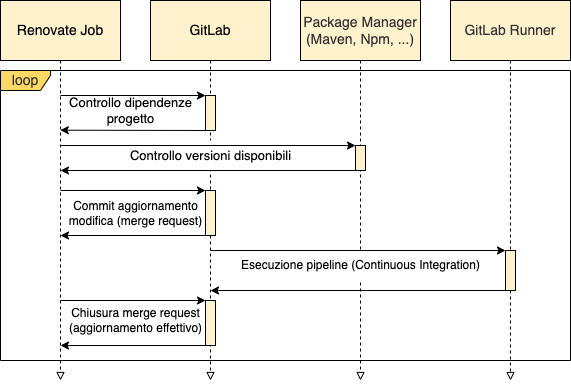
\includegraphics[width=0.85\textwidth]{img/renovate-uml-sequenza.png}
    \caption{Sequenza di aggiornamento automatico delle dipendenze con Renovate e GitLab Runner}
    \label{renovaflow}
\end{figure}

Tipicamente l'aggiornamento automatico avviene per versioni \textit{patch} e \textit{minor}, ovvero per quegli aggiornamenti che spesso non presentano \textit{breaking changes}: in tutti gli altri casi (\textit{major}) è necessaria l'approvazione manuale da parte di uno sviluppatore.

Il comportamento di Renovate può essere configurato ad-hoc per le diverse esigenze di ogni progetto tramite un apposito file, come quello seguente\footnote{\href{https://github.com/paganellif/DevOps-per-applicazioni-mobile-un-caso-di-studio-industriale/blob/5-automazione-del-processo-di-sviluppo/renovate.json}{https://github.com/paganellif/DevOps-per-applicazioni-mobile-un-caso-di-studio-industriale/blob/5-automazione-del-processo-di-sviluppo/renovate.json}}, versionato insieme al codice.

\begin{listing}[H]
    \inputminted{json}{code/renovate.json}
    \caption{Configurazione custom di un progetto Android per l'aggiornamento automatico delle dipendenze con Renovate}
\end{listing}

\section{Continuous Delivery}
Le precedenti fasi di integrazione continua, se completate con successo, restituiscono come output il pacchetto contenente tutte le informazioni utili alla stabilizzazione e alla distribuzione della applicazione. Nel caso dello sviluppo di applicazioni multipiattaforma con KMM bisogna considerare che le due applicazioni potrebbero essere rilasciate singolarmente, ad esempio a fronte di una modifica all'interfaccia grafica della sola versione Android, oppure essere rilasciate entrambe, tipicamente a causa di una modifica della logica applicativa che è condivisa dalle due applicazioni.

Data in input l'applicazione da distribuire è necessario svolgere una serie di operazioni, comuni ad entrambe le piattaforme Android e iOS, le quali richiedono considerazioni differenti dagli aspetti del normale sviluppo software, come (\textit{i}) l'identificazione ai servizi di distribuzione, (\textit{ii}) l'ottenimento dei permessi per l'utilizzo di certe API (creazione API-key), (\textit{iii}) la creazione dei certificati per la firma del codice (\textit{code signing}) e (\textit{iv}) la definizione dei gruppi di tester~\cite{mednieks2011programming}. Tutti questi sotto-task della fase di Continuous Delivery sono svolti sfruttando i servizi cloud forniti da Google e Apple per le relative piattaforme proprietarie, come anticipato nel capitolo \ref{ch:app-multiplatform}.

\subsection{Google Play Console}
A differenza delle applicazioni iOS, le quali richiedono due strumenti separati per la loro stabilizzazione e distribuzione, le applicazioni Android vengono gestite interamente da una unica piattaforma chiamata \textit{Google Play Console}. Tramite il concetto di promozione una specifica versione di applicazione viene promossa a versione \textit{alpha}, promossa da \textit{alpha} a \textit{beta} o da \textit{beta} a \textit{produzione}, quest'ultima equivalente alla pubblicazione sul marketplace \textit{Google Play Store}.

Per poter abilitare il sistema di automazione ad eseguire la fase di delivery per la piattaforma Android sono richiesti i seguenti passaggi:

\begin{itemize}
    \item Creazione account \textit{Google Developer}.
    \item Creazione scheletro iniziale della applicazione sul portale Google Play Console. Devono essere compilati questionari obbligatori, come quello per la classificazione PEGI\footnote{\href{https://pegi.info/it}{https://pegi.info/it}}, create le mailing list per gli alpha/beta tester e impostate preferenze come la monetizzazione della applicazione e la presenza di pubblicità/annunci.
    \item Creazione Service Account per autenticare le chiamate alle API Google. Queste informazioni devono essere inserite in GitLab per poter essere usate durante l'esecuzione delle pipeline.
    \item Creazione chiavi e certificati, in formato \textit{Java KeyStore} (jks) per la firma del codice. Tale formato deve essere codificato in esadecimale per poter essere utilizzato in GitLab al fine di automatizzare il processo di firma del codice. Il seguente script\footnote{\href{https://github.com/paganellif/DevOps-per-applicazioni-mobile-un-caso-di-studio-industriale/blob/5-automazione-del-processo-di-sviluppo/jks-android-gitlab.sh}{https://github.com/paganellif/DevOps-per-applicazioni-mobile-un-caso-di-studio-industriale/blob/5-automazione-del-processo-di-sviluppo/jks-android-gitlab.sh}} bash mostra un esempio per la creazione, codifica e decodifica della chiave jks:

    \begin{listing}[H]
        \inputminted{bash}{code/jks-android-gitlab.sh}
        \caption{Comandi bash d'esempio per la creazione, codifica e decodifica di una chiave in formato jks}
    \end{listing}
\end{itemize}

\subsection{App Store Connect}
Nell'ecosistema Apple non esiste il concetto di promozione di versione. La tipologia di rilascio viene discriminata in base al gruppo di tester target definiti sul portale \textit{Testflight}, nello specifico il gruppo \textit{Internal Tester} comprende i tester con accesso alla versione \textit{alpha} mentre il gruppo \textit{External Tester} quelli con accesso alla versione \textit{beta}. 

La sequenza di step necessari a configurare il sistema di automazione è molto simile a quella sopra descritta per le applicazioni Android:

\begin{itemize}
    \item Creazione account \textit{Apple Developer}.
    \item Creazione scheletro iniziale della applicazione sul portale App Store Connect: anche in questo caso devono essere compilati questionari obbligatori e impostate le preferenze analoghe al caso Android.
    \item Creazione gruppi per i tester interni ed esterni sul portale Testflight.
    \item Creazione API key\footnote{\href{https://docs.fastlane.tools/app-store-connect-api/\#using-fastlane-api-key-json-file}{https://docs.fastlane.tools/app-store-connect-api/\#using-fastlane-api-key-json-file}} per l'autenticazione ai servizi Apple e App-Specific Password per l'autenticazione del tool Fastlane. Come per i servizi Google, anche in questo caso è necessario inserire la chiave in GitLab per poterla utilizzare durante l'esecuzione della pipeline.
    \item Creazione certificato di tipo \textit{iOS Distribution} (Certificate Signing Request) e provisioning file del tipo \textit{App Store} per il processo di firma del codice. In questo caso non è necessario inserire le informazioni su GitLab perchè vengono automaticamente ottenute dal tool Fastlane autenticandosi ai servizi Apple.
\end{itemize}

\subsection{Alpha/Beta Release}
Considerando il modello di branching definito (fig. \ref{branching}), ognuno dei tre branch principali corrisponde ad un ambiente e quindi ad un preciso target di utilizzatori. Nel caso del branch di sviluppo principale \textit{dev} le applicazioni vengono rilasciate a scopo di testing interno da parte di figure tecniche tipicamente coinvolte nello sviluppo. 

Per rendere più veloce questa prima fase di stabilizzazione, dato che non vengono coinvolte persone esterne, sia Google che Apple permettono la distribuzione diretta senza il loro intervento per lo svolgimento del processo di \textit{App Review}. Il discorso cambia invece per tutte le altre fasi di delivery: la applicazione deve essere revisionata e approvata prima di poter procedere sia per il rilascio in \textit{beta} che per la vera e propria pubblicazione sui marketplace.

Il seguente codice\footnote{\href{https://github.com/paganellif/DevOps-per-applicazioni-mobile-un-caso-di-studio-industriale/blob/5-automazione-del-processo-di-sviluppo/kmm-templates/kmm-release.yml}{https://github.com/paganellif/DevOps-per-applicazioni-mobile-un-caso-di-studio-industriale/blob/5-automazione-del-processo-di-sviluppo/kmm-templates/kmm-release.yml}} definisce il job base per la distribuzione in versione \textit{alpha} di una applicazione Android:

\begin{listing}[H]
    \inputminted{yaml}{code/android-alpha-release-job.yaml}
    \caption{Job base per il rilascio in versione \textit{alpha} della applicazione Android}
\end{listing}

\begin{figure}[H]
    \centering
    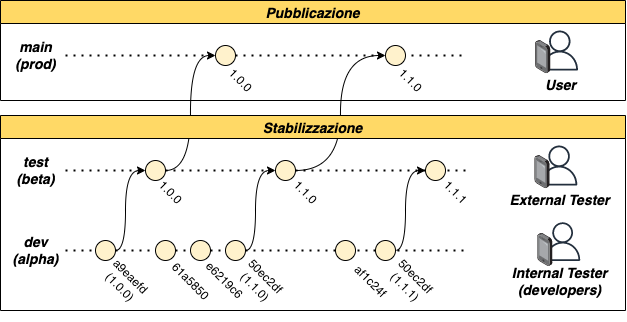
\includegraphics[width=0.75\textwidth]{img/release-flow.png}
    \caption{Stage, job e artefatti associati agli eventi sui branch che compongono l'intera pipeline}
    \label{release-alpha-beta-flow}
\end{figure}

\section{Continuous Inspection}
L'ultimo requisito del processo mancante è la fase di analisi automatica del codice sviluppato. Come descritto nel capitolo \ref{ch:devops} la pratica di Continuous Inspection può comprendere tantissime tecniche di analisi, tra cui quelle implementate nel caso di studio industriale che sono l'analisi statica (SAST) e l'analisi delle dipendenze (SCA).

\subsection{Composizione software}
Con composizione software si intende l'insieme di codice sviluppato da terze parti e che viene incluso all'interno della applicazione, tipicamente sotto forma di import di librerie, dette dipendenze. Queste dipendenze includono a loro volta altre dipendenze e potrebbero introdurre vulnerabilità nella applicazione che le utilizza: per questo motivo è necessario analizzare le dipendenze al fine di individuare le vulnerabilità ed essere tempestivi nel loro aggiornamento non appena vengono rilasciate delle patch di sicurezza. 

Il tool adottato a livello aziendale per effettuare questa tipologia di analisi è \textit{DependencyCheck}\footnote{\href{https://github.com/jeremylong/DependencyCheck}{https://github.com/jeremylong/DependencyCheck}}, un tool open-source rilasciato e mantenuto da OWASP\footnote{\href{https://owasp.org/}{https://owasp.org/}}, disponbile come plugin Gradle, binario eseguibile e immagine Docker. Uno dei principali punti di forza di questo tool è la possibilità di analizzare più progetti di diversa natura, come applicazioni Android e iOS, senza la necessità di configurazioni complesse\footnote{\href{https://github.com/paganellif/DevOps-per-applicazioni-mobile-un-caso-di-studio-industriale/blob/5-automazione-del-processo-di-sviluppo/kmm-templates/kmm-analysis.yml}{https://github.com/paganellif/DevOps-per-applicazioni-mobile-un-caso-di-studio-industriale/blob/5-automazione-del-processo-di-sviluppo/kmm-templates/kmm-analysis.yml}}:

\begin{listing}[H]
    \inputminted{yaml}{code/depcheck-job.yaml}
    \caption{Job base dedicato alla analisi delle dipendenze sia Android che iOS tramite il tool OWASP DependencyCheck}
\end{listing}

\subsection{Analisi statica}
Per quanto riguarda l'analisi statica del codice non è possibile invece un livello di semplicità di configurazione come quello dell'analisi delle dipendenze. Gli strumenti necessari per questa fase di analisi dipendono fortemente dalle tecnologie adottate e dalle piattaforme target. I moduli della applicazione KMM, ovvero (\textit{i}) applicazione Android, (\textit{ii}) applicazione iOS e (\textit{iii}) logica condivisa, devono essere considerati come moduli separati per utilizzare i seguenti strumenti di analisi individuati:

\begin{itemize}
    \item \textbf{Android Lint}  - Tool per l'analisi statica di applicazioni Android, disponibile come binario e plugin Gradle (a partire dalla versione 16 ADT\footnote{Android Development Tools}).
    \item \textbf{Detekt}  - Tool specifico per l'analisi statica di codice Kotlin, disponibile come binario eseguibile e plugin Gradle.
    \item \textbf{SwiftLint} - Tool specifico per l'analisi statica di codice Swift, disponibile come binario eseguibile e dipendenza CocoaPods.
    \item \textbf{SonarQube} - Client tool per l'interazione con il sistema aziendale SonarQube, disponibile come binario eseguibile e plugin Gradle.
\end{itemize}

Il seguente codice\footnote{\href{https://github.com/paganellif/DevOps-per-applicazioni-mobile-un-caso-di-studio-industriale/blob/5-automazione-del-processo-di-sviluppo/kmm-templates/kmm-analysis.yml}{https://github.com/paganellif/DevOps-per-applicazioni-mobile-un-caso-di-studio-industriale/blob/5-automazione-del-processo-di-sviluppo/kmm-templates/kmm-analysis.yml}} mostra l'utilizzo dello strumento SwiftLint per l'analisi statica di applicazioni iOS tramite il job base schedulato:

\begin{listing}[H]
    \inputminted{yaml}{code/ios-sast-job.yaml}
    \caption{Job base dedicato alla analisi statica del codice Swift della applicazione iOS}
\end{listing}

\subsection{Schedulazione Job}
Le fasi di analisi del codice possono essere introdotte nel processo di sviluppo distinguendo due modalità di esecuzione:

\begin{itemize}
    \item \textbf{Sincrona} - L'analisi del codice viene eseguita ad ogni commit su uno specifico branch (in questo caso \textit{dev}). Il vantaggio consiste nella ricezione di un feedback più rapido sulla modifica apportata al codice mentre lo svantaggio è dato da un incremento considerevole nel tempo di esecuzione di ogni pipeline.
    \item \textbf{Asincrona} - Tramite la schedulazione delle fasi di analisi in un momento diverso da quello in cui viene apportata la modifica al codice è possibile sia ridurre i tempi di esecuzione delle pipeline che ottenere un feedback cumulativo sull'insieme delle modifiche apportate tra due esecuzioni delle pipeline di analisi del codice. Ad esempio, schedulando alla mezzanotte di ogni giorno l'esecuzione delle fasi di analisi, è possibile accedere al portale SonarQube all'inizio della giornata lavorativa successiva e pianificare gli interventi di risoluzione degli eventuali bug introdotti nella giornata precedente.
\end{itemize}

\begin{figure}[H]
    \centering
    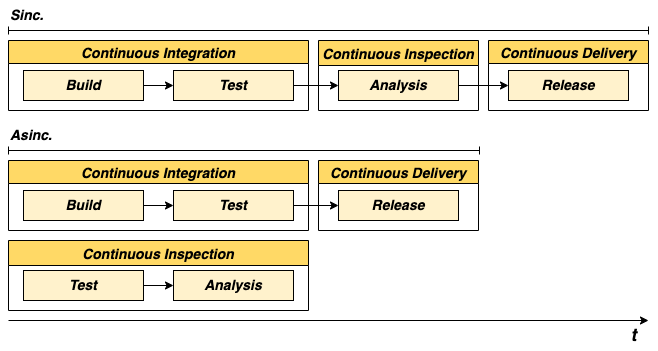
\includegraphics[width=0.82\textwidth]{img/inspection-sync-async.png}
    \caption{Confronto tra esecuzione sincrona e asincrona della fase di analisi}
    \label{inspection-sync-async}
\end{figure}

\begin{figure}[H]
    \centering
    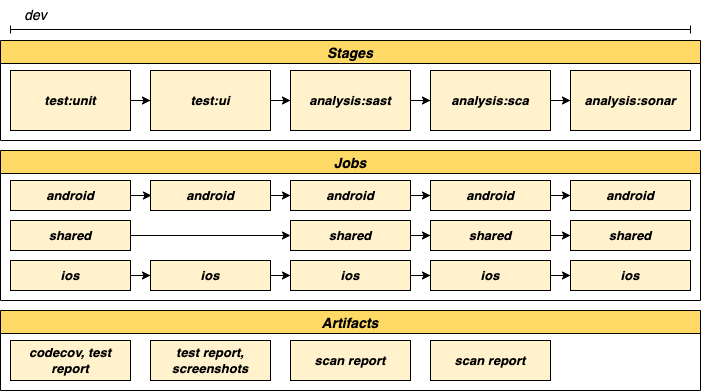
\includegraphics[width=0.82\textwidth]{img/inspection-pipeline.png}
    \caption{Struttura della seconda pipeline schedulata per l'analisi del codice}
\end{figure}

La modalità di esecuzione scelta per la fase di Continuous Inspection è quella asincrona per i suoi vantaggi, preferiti dalla maggior parte dei team di sviluppo in azienda rispetto a quelli dell'esecuzione sincrona. E' necessario dunque schedulare una seconda pipeline in grado di: (\textit{i}) eseguire i test, (\textit{ii}) eseguire l'analisi statica del codice, (\textit{iii}) eseguire l'analisi delle dipendenze e (\textit{iv}) collezionare tutti i report prodotti dalle fasi precedenti al fine di caricarli sul sistema aziendale SonarQube per la gestione centralizzata delle vulnerabilità.